\documentclass{beamer}
\usepackage[utf8]{inputenc}

\usepackage{amsmath}
\usepackage{graphicx}
\usepackage{url}
\usepackage{fancyvrb}
\usepackage{xcolor}

\usetheme{Antibes}
\usecolortheme{whale}
\usepackage{lmodern}

\usepackage{listings}
\usepackage{color}

\definecolor{codegreen}{rgb}{0,0.6,0}
\definecolor{codegray}{rgb}{0.5,0.5,0.5}
\definecolor{codepurple}{rgb}{0.58,0,0.82}
\definecolor{backcolour}{rgb}{0.95,0.95,0.92}

\mode<presentation>

\definecolor{orange}{HTML}{BC2E07}

\usepackage{hyperref}
\hypersetup{
    colorlinks,
    linkcolor=orange,
    urlcolor=blue
}

\lstdefinestyle{mystyle}{
    language=C++,
    basicstyle=\ttfamily\footnotesize,
    backgroundcolor=\color{backcolour},
    commentstyle=\color{codegreen},
    keywordstyle=\color{magenta},
    numberstyle=\tiny\color{codegray},
    stringstyle=\color{codepurple},
    breakatwhitespace=false,
    breaklines=true,
    captionpos=b,
    keepspaces=true,
    numbers=left,
    numbersep=5pt,
    showspaces=false,
    showstringspaces=false,
    showtabs=false,
    tabsize=2
}

\title{Lab \# 5: Relational Operators, Logical Operators and Decisions}
\subtitle{EC-102 -- Computer Systems and Programming}

\author{Usama Wajhi}
\institute{School of Mechanical and Manufacturing Engineering (SMME), \\ National University of Sciences and Technology (NUST)}
\date{\today}

\begin{document}
\begin{frame}
    \titlepage
\end{frame}

\begin{frame}
    \frametitle{Outline}
    \begin{columns}
        \column{0.5\textwidth}
        \begin{small}
        \tableofcontents
        \end{small}
        
        \column{0.5\textwidth}
        \begin{figure}
            \centering
            
\includegraphics[scale=0.28]{comment}
        \end{figure}
    \end{columns}
\end{frame}

\begin{frame}
    \frametitle{Relational Operators -- Why do we need them?}
    \section{Relational Operators} % (fold)
    \label{sec:relational_operators}
    \subsection{Importance} % (fold)
    \label{sub:importance}
    \begin{columns}
        \column{0.6\textwidth}
        \begin{small}
         \begin{itemize}
            \item Most programs decide what to do in response to changing circumstances
            \item The flow of control jumps from one part of the program to another in response to such events
            \item Program statements that cause such jumps are called \textbf{control statements} e.g. decisions and loops
            \item How many times a loop is executed or whether a decision results in the execution of a section of code depends on whether certain expressions turn out to be \textit{true} or \textit{false}
        \end{itemize}
        \end{small}
       
        \column{0.4\textwidth}
        \begin{figure}
            \centering
            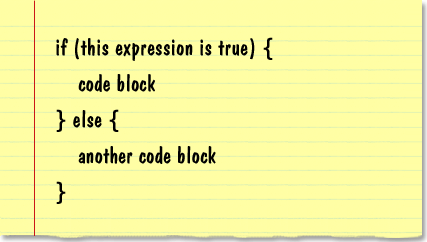
\includegraphics[scale=0.35]{if_else}
        \end{figure}
        \begin{figure}
            \centering
            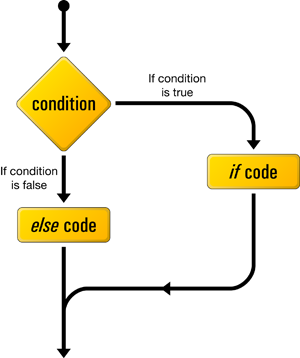
\includegraphics[scale=0.3]{ifelse}
        \end{figure}
    \end{columns}
\end{frame}

\begin{frame}
    \frametitle{Relational Operators -- What are they?}
    \subsection{Definition} % (fold)
    \label{sub:definition}
    \begin{itemize}
        \item A relational operator compares two values
        \item The comparison involves such relationships as equal-to, lesser-than, and greater-than
        \item The result of the comparison is true or false
    \end{itemize}
\end{frame}

\begin{frame}[fragile]
    \frametitle{Relational Operators -- Examples}
    \subsection{Examples} % (fold)
    \label{sub:examples}
    \textbf{Example \# 1}
    \lstset{style=mystyle}
    \begin{lstlisting}
// this program demonstrates relational operators in a comparison of int, float and char constants
#include <iostream>
using namespace std;
int main(){
    cout << (10 > 20) << endl; // false
    cout << (10 < 20) << endl; // true
    cout << (20 == 20) << endl; // true

    cout << (20.5 > 20.0) << endl; // true
    cout << (20.5 == 2.5) << endl; // false

    cout << ('a' == 'a') << endl; // true
    cout << ('a' > 'b') << endl; // false
    return 0;
}\end{lstlisting}
\end{frame}

\begin{frame}[fragile]
    \frametitle{Relational Operators -- Examples}
    \textbf{Example \# 2}
    \lstset{style=mystyle}
    \begin{lstlisting}
//  relational operators in a comparison of int variables
#include <iostream>
using namespace std;
int main(){
    int jane = 44; // assignment statement
    int harry = 12;

    cout << (jane == harry) << endl;
    cout << (harry <= 12) << endl;
    cout << (jane > harry) << endl;
    cout << (jane >= 44) << endl;
    cout << (harry != 12) << endl;
    cout << (7 < harry) << endl;
    return 0;
}\end{lstlisting}
\end{frame}

\begin{frame}
    \frametitle{Relational Operators in C++}
    \subsection{Relational Operators in C++} % (fold)
    \label{sub:a_complete_list}
    Here's a complete list of C++ relational operators,
    \begin{table}
        \begin{tabular}{c | l}
        Operator & Meaning \\
        \hline \hline
        $>$ & Greater than \\
        $<$ & Lesser than\\
        $==$ & Equal to\\
        $!=$ & Not equal to\\
        $>=$ & Greater than or equal to\\
        $<=$ & Lesser than or equal to
        \end{tabular}
    \end{table}
\end{frame}

\begin{frame}
    \frametitle{Logical Operators -- Why do we need them?}
    \section{Logical Operators} % (fold)
    \label{sec:logical_operators}
    \subsection{Importance} % (fold)
    \label{sub:importance_2}
    \begin{columns}
        \column{0.6\textwidth}
        \begin{itemize}
            \item While relational operators can be used to test whether a particular condition is true or false, they can only test one condition at a time
            \item Often we need to know whether multiple conditions are true at once
            \item Other times, we need to know whether any one of the multiple conditions is true
        \end{itemize}
        \column{0.4\textwidth}
            \begin{figure}
                \centering
                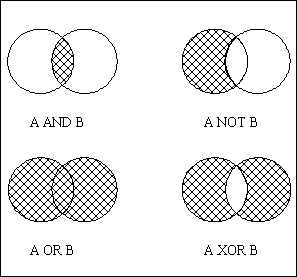
\includegraphics[scale=0.6]{venn.png}
            \end{figure}
    \end{columns}
\end{frame}

\begin{frame}
    \frametitle{Logical Operators -- What are they?}
    \subsection{Definition} % (fold)
    \label{sub:definition_2}
    \begin{itemize}
        \item A relational operator is used to combine two Boolean expressions
        \item For example, to check whether a number x entered by the user satisfies the expression 20 $<$ x $<$ 30, we would need to logically connect both the expressions \texttt{(x $>$ 20)} and \texttt{(x $<$ 30)} and see if there combination yields true or false
        \item The logical connection in this case is the word AND
        \item The result of logical operation is either true or false
    \end{itemize}
\end{frame}

\begin{frame}
    \frametitle{Logical Operators in C++}
    \subsection{Logical Operators in C++} % (fold)
    \label{sub:a_complete_list_2}
    Here's a complete list of C++ logical operators,
    \begin{table}
        \begin{tabular}{c | l}
        Operator & Meaning \\
        \hline \hline
        $\&\&$ & AND \\
        $||$ & OR\\
        $!$ & NOT
        \end{tabular}
    \end{table}
\end{frame}

\begin{frame}
    \frametitle{Logical AND Operator ($\&\&$)}
    \subsubsection{AND Operator} % (fold)
    \label{ssub:and_operator}
    \begin{table}
        \begin{tabular}{c | c | c}
        Expression 1 & Expression 2 & Expression 1 $\&\&$ Expression 2 \\
        \hline \hline
        false & false & false\\
        false & true & false\\
        true & false & false\\
        true & true & true
        \end{tabular}
    \end{table}
\end{frame}

\begin{frame}
    \frametitle{Logical OR Operator ($||$)}
    \subsubsection{OR Operator} % (fold)
    \label{ssub:or_operator}
    \begin{table}
        \begin{tabular}{c | c | c}
        Expression 1 & Expression 2 & Expression 1 $||$ Expression 2 \\
        \hline \hline
        false & false & false\\
        false & true & true\\
        true & false & true\\
        true & true & true
        \end{tabular}
    \end{table}
\end{frame}

\begin{frame}
    \frametitle{Logical NOT Operator (!)}
    \subsubsection{NOT Operator} % (fold)
    \label{ssub:not_operator}
    \begin{itemize}
        \item Logical NOT operator is a unary operator
        \item It can be used to reverse the meaning of a Boolean expression
    \end{itemize}
    \begin{table}
        \begin{tabular}{c | c}
        Expression & !Expression\\
        \hline \hline
        false & true\\
        true & false\\
        \end{tabular}
    \end{table}
\end{frame}

\begin{frame}[fragile]
    \frametitle{Logical Operators -- Example}
    \subsection{Examples} % (fold)
    \label{sub:examples_2}
    \lstset{style=mystyle}
    \begin{lstlisting}
// this program demonstrates logical operators
#include <iostream>
using namespace std;
int main()
{
    int jane = 44;
    int harry = 12;

    cout << (jane == harry && harry <= 12) << endl;
    cout << (jane == harry || harry <= 12) << endl;
    cout << !(jane == harry) << endl;

    cout << (jane > harry && jane >= 44) << endl;
    cout << (jane > harry || jane >= 44) << endl;
    cout << !(jane > harry || jane >= 44) << endl;
    return 0;
}\end{lstlisting}
\end{frame}

\begin{frame}
    \frametitle{Decision Making}
    \section{Decision Making in C++} % (fold)
    \label{sec:decision_making}
    \subsection{Introduction} % (fold)
    \label{sub:introduction}
    \begin{itemize}
        \item Decision making is about deciding the order of execution of statements based on certain conditions
        \item These statements require the programmer to specify:
        \begin{itemize}
            \item One or more expressions to be evaluated or tested by the program along with
            \item One or more statements to be executed if the condition turns out to be true, and optionally
            \item One or more statements to be executed if the expression turns out to be false
        \end{itemize}
    \end{itemize}
\end{frame}

\begin{frame}
    \frametitle{Decision Making in C++}
    \subsection{Decision Making in C++} % (fold)
    \label{sub:decision_making_in_c_}
    \begin{itemize}
        \item Decisions can be made in C++ in many ways. The most important is with the \texttt{if...else} statement. This statement can also be used without the \texttt{else}, as a simple \texttt{if} statement.
        \item Another decision statement, \texttt{switch}, creates branches for the multiple alternative sections of code, depending on the value of a single variable
    \end{itemize}
\end{frame}

\begin{frame}[fragile]
    \frametitle{The \texttt{if} Statement}
    \subsubsection{The \texttt{if} Statement} % (fold)
    \label{ssub:the_if}
    \begin{columns}
    \column{0.6\textwidth}
    \textbf{Algorithm}
    \begin{enumerate}
        \item Start
        \item Declare variable x
        \item Read value of x
        \item If x is greater than 100 then display ``The number is greater than 100''
        \item Stop
    \end{enumerate}
    \column{0.40\textwidth}
    \textbf{Flowchart}
    \begin{figure}
        \centering
        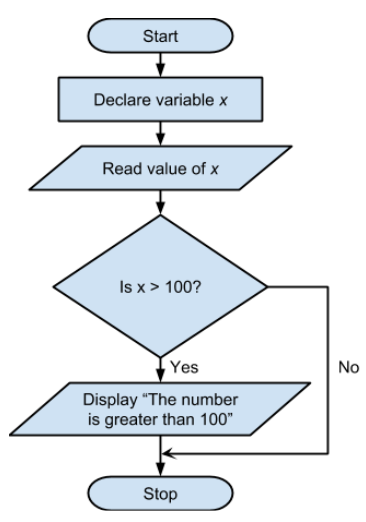
\includegraphics[scale=0.47]{flowchart}
    \end{figure}
    \end{columns}
\end{frame}

\begin{frame}[fragile]
    \frametitle{The \texttt{if} Statement}
    \textbf{Code}
    \lstset{style=mystyle}
    \begin{lstlisting}
// this program demonstrates IF statement
#include <iostream>
using namespace std;
int main()
{
    int x;

    cout << "Enter a number: ";
    cin >> x;

    if(x > 100)
    {
        cout << "That number is greater than 100\n";
    }

    return 0;
}\end{lstlisting}

\end{frame}

\begin{frame}[fragile]
    \frametitle{The \texttt{if...else} Statement}
    \subsubsection{The \texttt{if...else} Statement} % (fold)
    \label{ssub:the_if_else}
    \begin{columns}
    \column{0.5\textwidth}
    \textbf{Algorithm}
    \begin{enumerate}
        \item Start
        \item Declare variable x
        \item Read value of x
        \item If x is greater than 100 then display ``The number is greater than 100''
        \item Else, display ``The number is not greater than 100''
        \item Stop
    \end{enumerate}
    \column{0.50\textwidth}
    \textbf{Flowchart}
    \begin{figure}
        \centering
        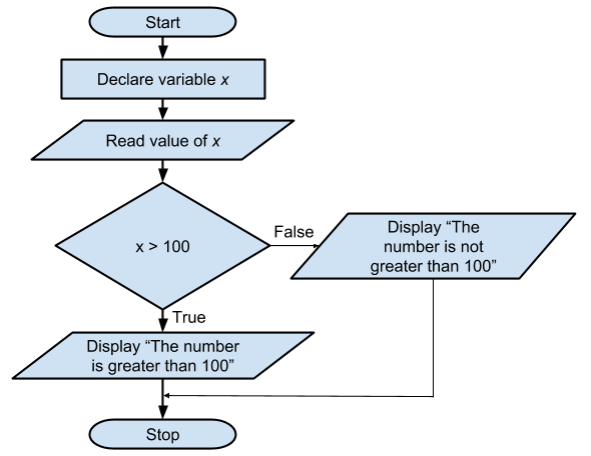
\includegraphics[scale=0.4]{flowchart2}
    \end{figure}
    \end{columns}
\end{frame}

\begin{frame}[fragile]
    \frametitle{The \texttt{if...else} Statement}
    \textbf{Code}
    \lstset{style=mystyle}
    \begin{lstlisting}
// this program demonstrates IF statement
#include <iostream>
using namespace std;
int main()
{
    int x;
    cout << "Enter a number: ";
    cin >> x;

    if(x > 100)
    {
        cout << "That number is greater than 100\n";
    }
    else
    {
        cout << "The number is not greater than 100\n";
    }
    return 0;
}\end{lstlisting}

\end{frame}

\begin{frame}{Programming Quiz}
Write a Program which works like an X-NOR operator.
    \begin{table}
        \begin{tabular}{c | c | c}
        x & y & x (XNOR) y \\
        \hline \hline
        0 & 0 & 1\\
        0 & 1 & 0\\
        1 & 0 & 0\\
        1 & 1 & 1
        \end{tabular}
    \end{table}(Time: 15 minutes)
	
\end{frame}
\end{document}